\chapter{Misure effettuate e dati sperimentali}
\label{capitolo5}
\thispagestyle{empty}

\textit{In questo Capitolo verranno presentati e commentati i risultati delle prove sperimentali svolte.}

\section{Metodologia proposta}
Per testare lo strumento e valutarne le prestazioni sono state effettuate tre differenti tipologie di prove.

La prima consiste nell'acquisire un certo numero di misure di un bersaglio fisso a distanza nota. La seconda tipologia, al contrario, si articola in due fasi. Inizialmente si acquisisce un campione della distanza del sensore da un bersaglio montato su una slitta motorizzata in grado di compiere spostamenti precisi; in seguito si procede spostando la slitta di una distanza nota, ripetendo il procedimento un numero prefissato di volte. Le due prove mirano a valutare differenti caratteristiche dello strumento: la precisione della misura e la sua accuratezza.

Queste prove sono state effettuate inizialmente ad una distanza prefissata di $50cm$ e ripetute ad ogni passo dello sviluppo dello strumento. A strumento ultimato sono state effettuate ulteriori misurazioni (a $20cm$ e a $90cm$), per valutare le prestazioni del prototipo finale su un range più vario di distanza.

La terza tipologia di prova, invece, si svolge mantenendo il bersaglio fisso ad una distanza prestabilita acquisendo un numero di campioni coerente con quello che lo strumento finale userà per fornire all'utente un singolo campione di distanza. In seguito si varia la distanza del bersaglio dal sensore e si ripete l'acquisizione. Lo scopo della prova è valutare empiricamente il range di misura dello strumento.

Per tutte le prove il fuoco del laser è stato mantenuto oltre la massima distanza misurata in ciascuna prova.

Di seguito sono descritte più nel dettaglio le metodologie di prove effettuate. Per confrontare i miglioramenti tra diverse implementazioni si è scelto di valutare la deviazione standard  (o incertezza) relativa della misura.

\begin{figure}  
  \begin{center}
  	%% TODO Cap5 Sistemare foto allestimento misura
    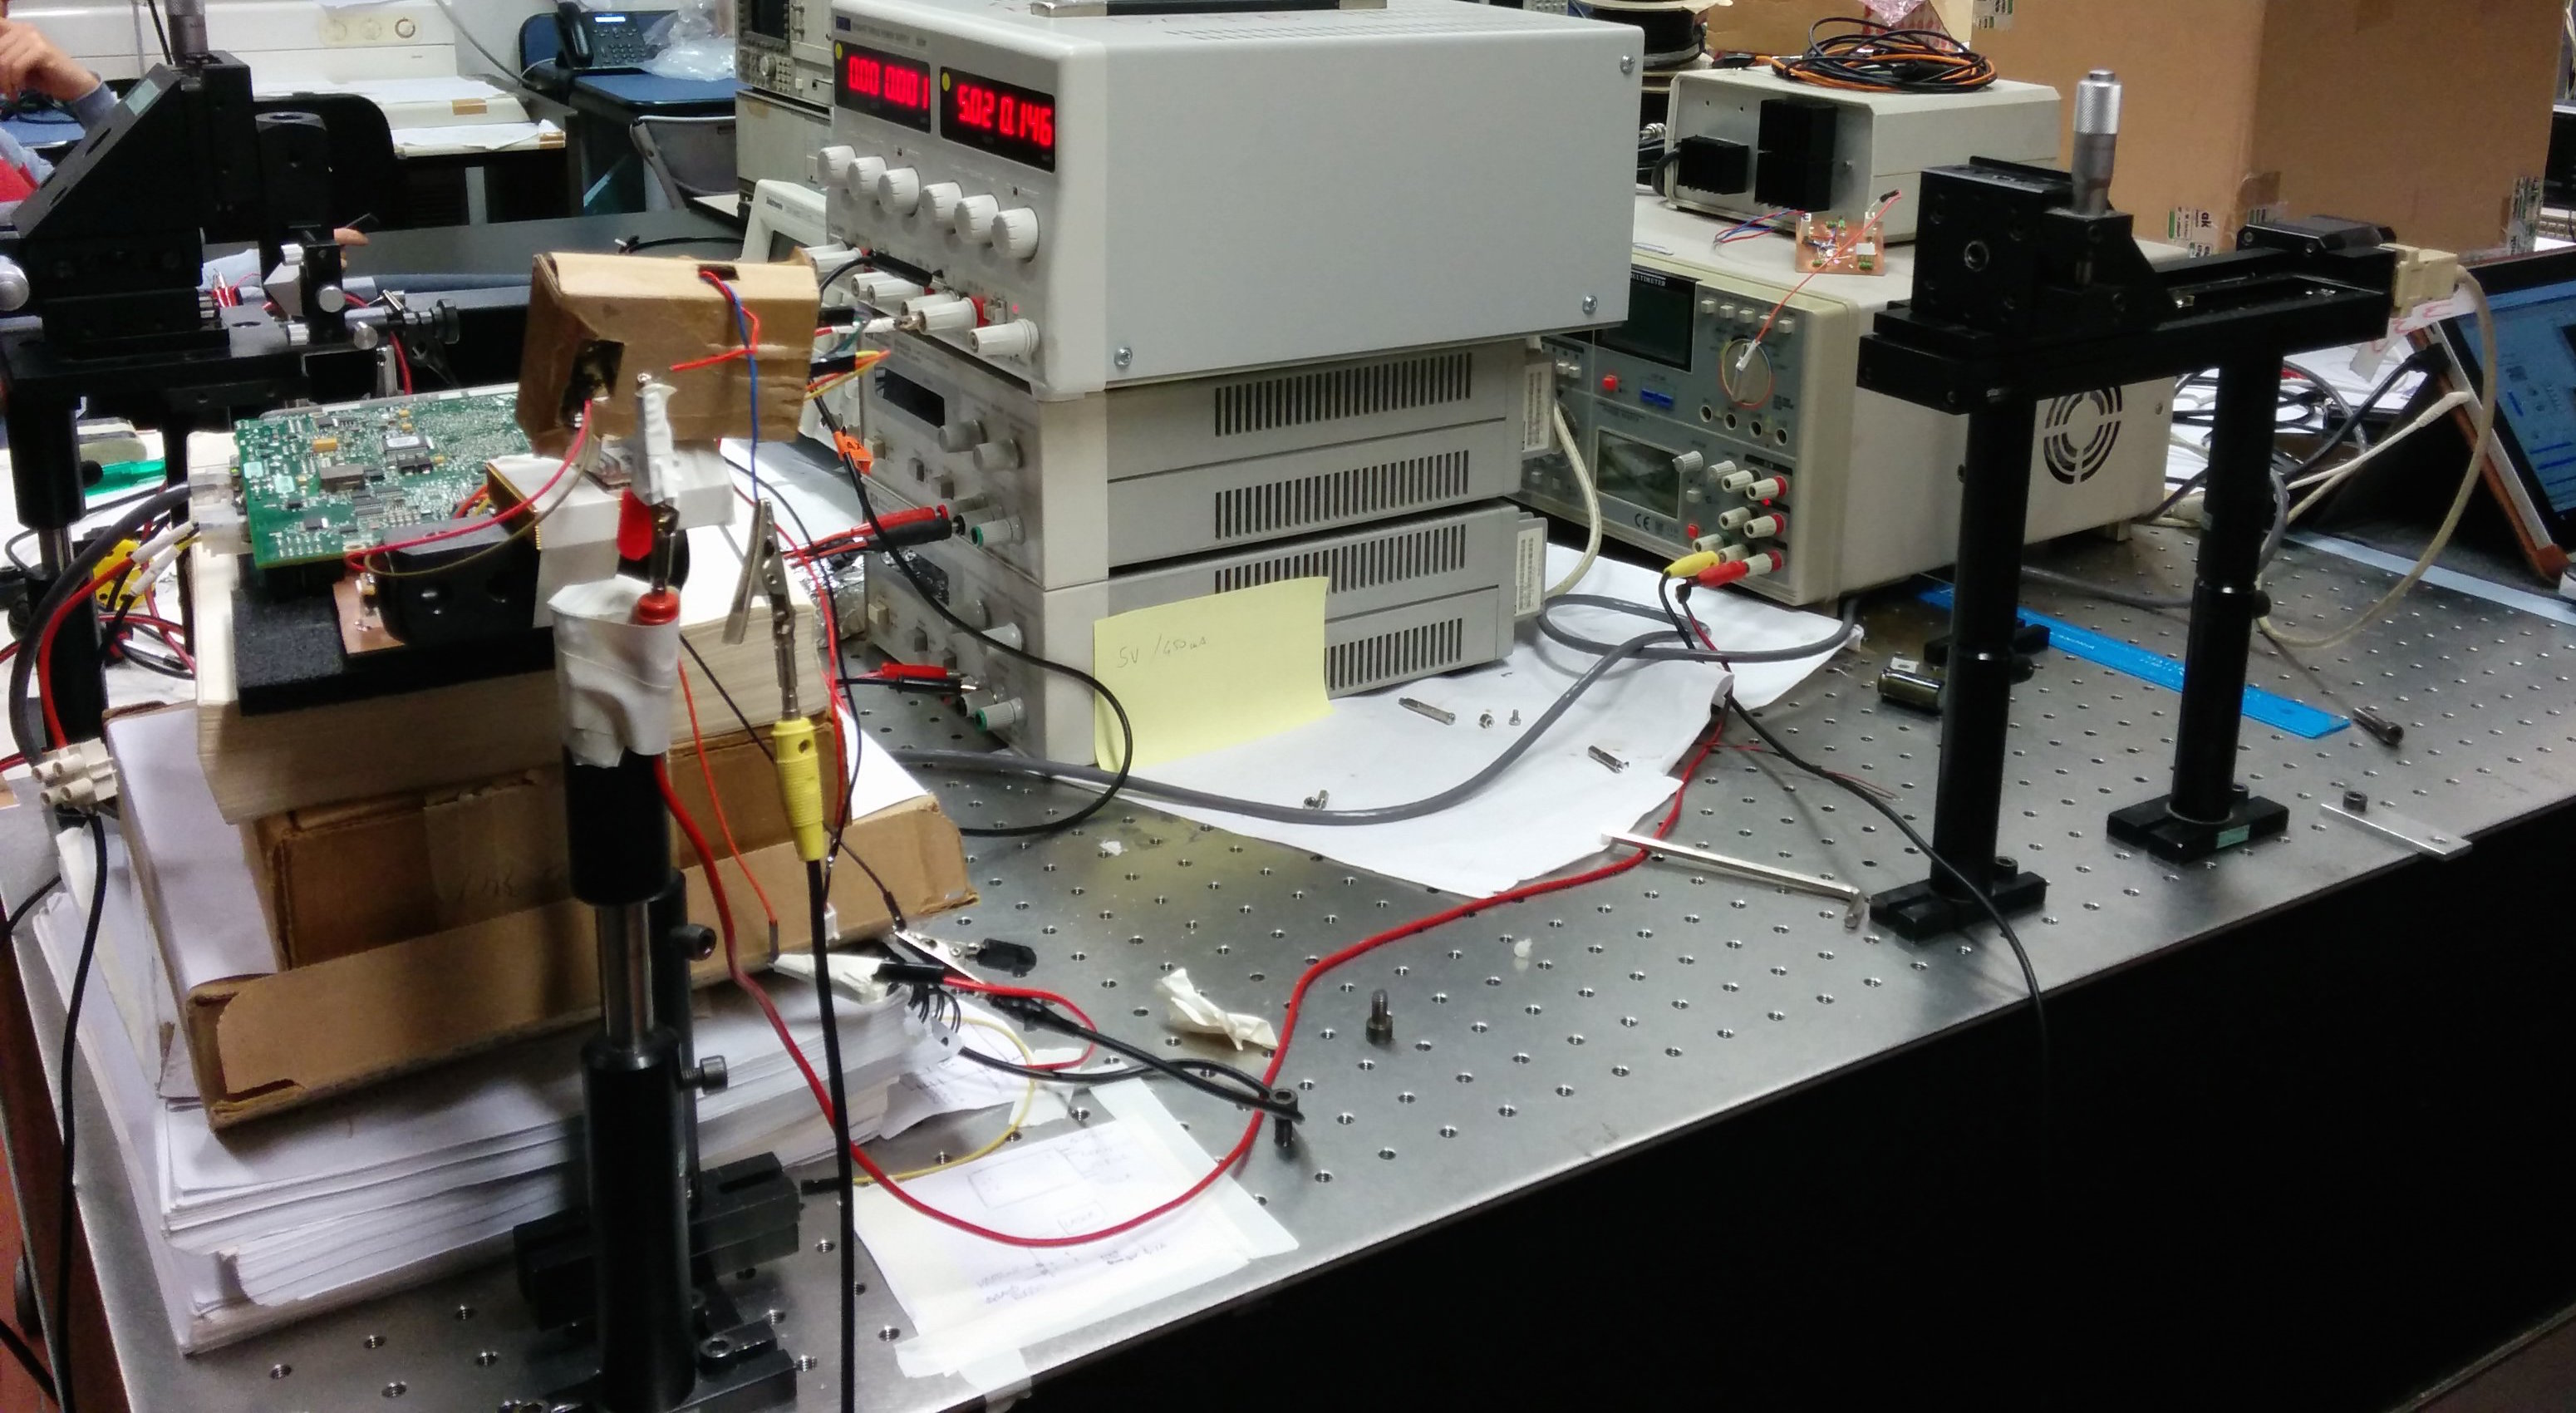
\includegraphics[scale=0.1]{cap5/allestimento}
    \caption{Allestimento della misura}
  \end{center}
\end{figure}

\subsection{Prova a bersaglio fisso}
La misura a bersaglio fisso è stata effettuata con il sensore fissato su di un tavolo ottico e puntato verso un bersaglio metallico nero, anch'esso fissato ad un tavolo ottico. L'uso del tavolo ottico si è reso necessario per minimizzare l'effetto delle vibrazioni.

Inizialmente si è lasciato in esecuzione il software che effettua la modulazione del laser, in modo da consentire al sensore di raggiungere una temperatura stabile, per minimizzare l'influenza del cambiamento di temperatura del laser sulla misura. Si è deciso di lasciare attiva la modulazione senza acquisire dati per $10$ minuti.

Con lo strumento ad una temperatura stabile si sono acquisiti $1000$ campioni della distanza dal bersaglio e se ne è valutata la media e la deviazione standard relativa. In questo modo è stato possibile valutare quanto è ampia l'oscillazione della misura rispetto alla media, e di determinare così la precisione dello strumento.

La misura si ritiene più precisa tanto minore è la sua deviazione standard relativa.

\subsection{Prova a bersaglio mobile}
La misura a bersaglio mobile è stata effettuata con un allestimento simile alla prova precedente. L'unica differenza è stato il fissaggio del bersaglio ad una slitta micrometrica, codice prodotto \textit{STANDA 8MT175-150}, uno strumento in grado di eseguire spostamenti dell'ordine dei micrometri, con una precisione di $0.31 \mu m$ \cite{standa}.

La prova si articola in due fasi:
\begin{enumerate}
	\item Acquisizione
	\item Spostamento
\end{enumerate}
Nella fase di acquisizione, con il bersaglio fermo, si acquisiscono $100$ campioni della distanza dal sensore. Di questi campioni si valutano media e deviazione standard relativa.
Nella fase di spostamento si allontana la slitta di $200 \mu m$ dal sensore. Si è scelto di utilizzare un passo di $200 \mu m$ perché consistente con la risoluzione dello strumento verificata nella prova a bersaglio fisso.

Queste due fasi sono ripetute per $15 \div 20$ volte, in modo da coprire una distanza totale di $3 \div 4mm$.

Lo scopo della prova è quello di valutare la linearità dello strumento rispetto allo spostamento del bersaglio. Per fare questo si valuta l'oscillazione della misura rispetto alla retta ideale dello spostamento; in particolare si valutano distanza picco-picco dell'errore della misura rispetto alla retta ideale e l'RMS (\textit{Root Mean Square}, valore quadratico medio).

L'errore di misura è calcolabile in modo semplice con la relazione:
\begin{equation}
	e = x_t - x 
\end{equation}
Dove con $x_t$ si intende il punto teorico appartenente alla retta ideale del valor medio, e con $x$ si intende il punto misurato dal sensore. 

La distanza picco-picco dell'errore è misurata come:
\begin{equation}
	e_{pp} = max(e) - min(e)
\end{equation}

I risultati migliori si ottengono quando si riscontrano distanze picco-picco ed RMS minori.

\subsection{Prova del range di misura}
La prova del range di misura si effettua con un allestimento identico alla prima prova, ma, al contrario di quest'ultima, i campioni acquisiti sono in numero minore, ovvero $100$. Il numero è stato scelto in modo coerente con il numero di campioni che lo strumento finale utilizzerà per fornire all'utente un singolo valore di distanza. 

Poiché lo scopo della prova è valutare il range di distanze in cui lo strumento è in grado di lavorare nei limiti di precisione desiderati, si ripete l'acquisizione dei campioni a diverse distanze dal sensore, partendo da $10cm$ e arrivando a $100$ cm, con passi di $10cm$ circa.

Sui $100$ campioni acquisiti si valutano media e deviazione standard relativa, e si ritiene soddisfacente la prestazione dello strumento quando la deviazione standard relativa fornita è minore di $10^{-3}$.

\section{Finestratura del segnale}
Come già discusso nel Capitolo \ref{capitolo4}, l'implementazione finale dello strumento genera un'onda triangolare che modula la sorgente laser in corrente. 

L'onda di modulazione triangolare generata e il segnale interferometrico in risposta dal laser, sono formati entrambi da $1250$ punti, $625$ per il semiperiodo di discesa della triangolare di modulazione e $625$ per il semiperiodo di salita. 
\begin{figure}  
  \begin{center}
  	%% TODO Cap5 Legenda nella figura?
    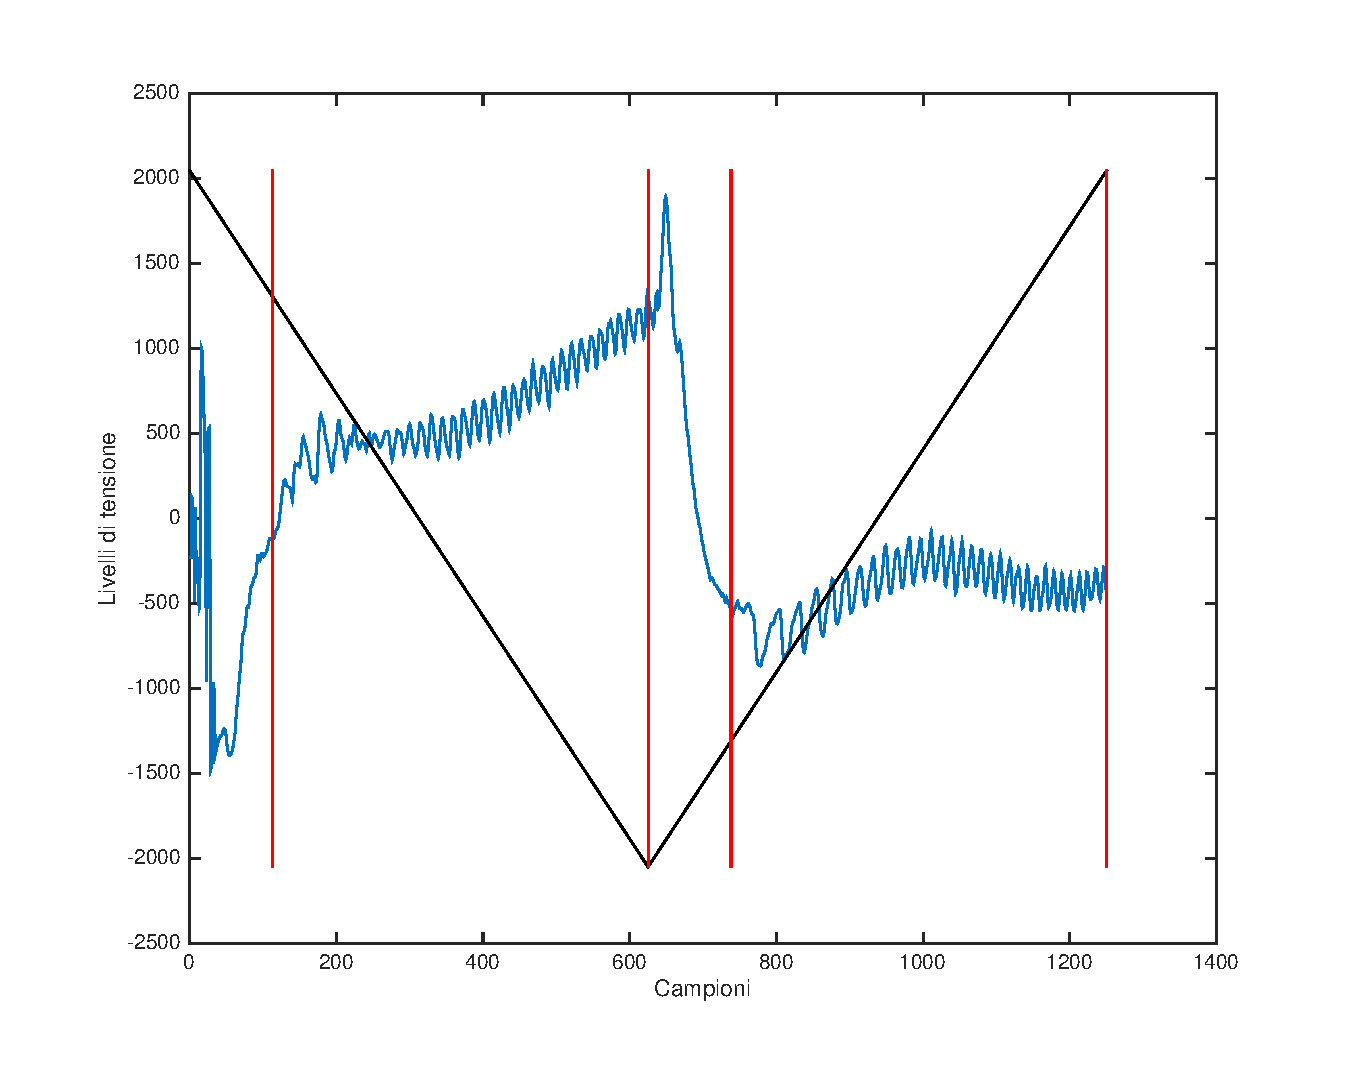
\includegraphics[scale=0.5]{cap5/segnaleinterf}
    \caption{Segnale interferometrico (blu) in un periodo di modulazione (nero)}
    \label{segnaleinterf}
  \end{center}
\end{figure}

Di questi $625$ punti soltanto $512$ contengono l'informazione utile per l'estrazione della frequenza interferometrica, poiché inizialmente si ha una parte di segnale influenzata dall'inversione del verso di polarizzazione del laser (Figura \ref{segnaleinterf}). 

Per l'estrazione del tono fondamentale del segnale si utilizza l'algoritmo di FFT interpolata a due punti con finestratura a $512$ punti.

Inoltre si sono valutate due differenti finestrature per il segnale, la finestratura rettangolare e quella di \textit{Hanning}.

Per determinare quale delle due finestrature utilizzare nell'implementazione finale dello strumento sono state realizzate prove a bersaglio fisso e a bersaglio mobile con modulazione triangolare a pendenza fissa.
\begin{figure}
\centering
\subfigure[Misure di distanza e media]
{\label{misfisso1a}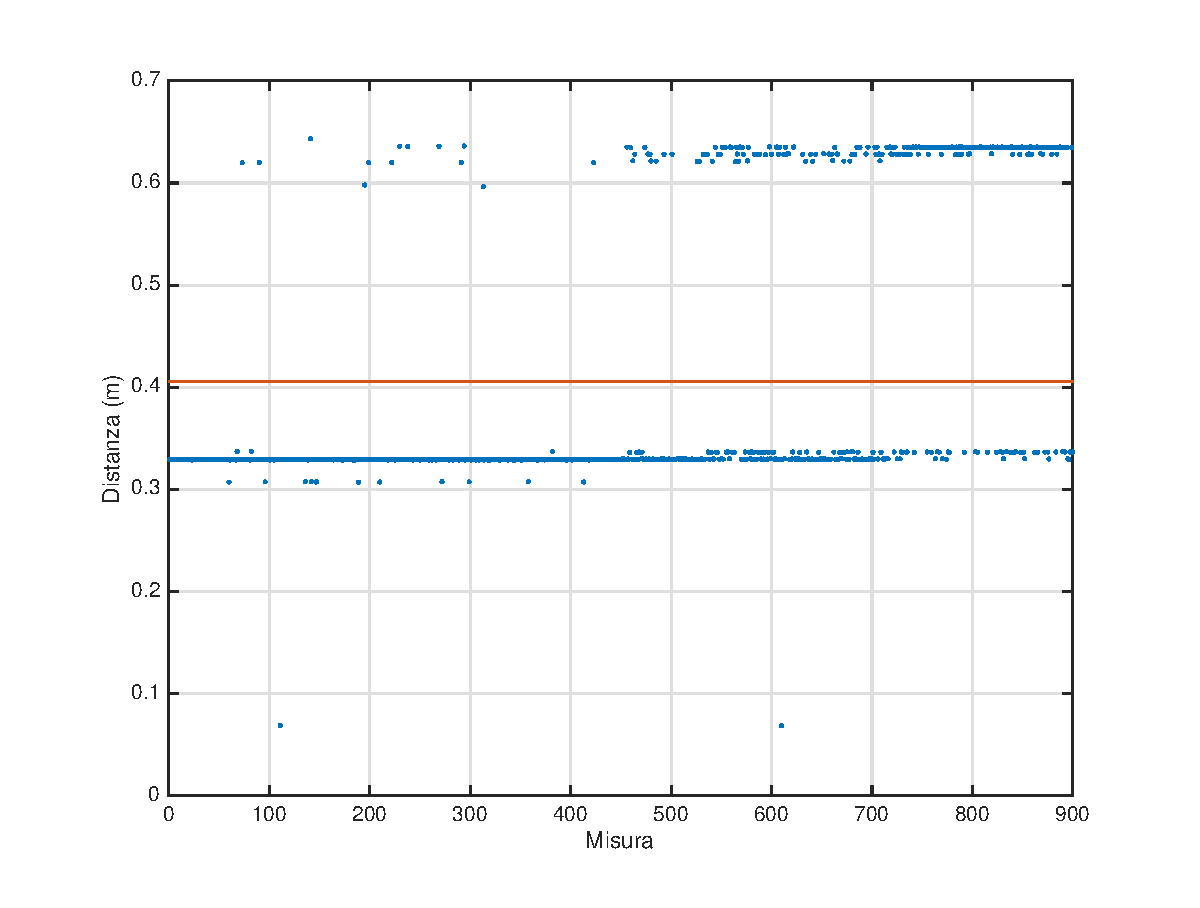
\includegraphics[scale=.5]{cap5/misfisso1a}}
\hspace{5mm}
\subfigure[Distribuzione dei valori misurati rispetto alla media]
{\label{misfisso1b}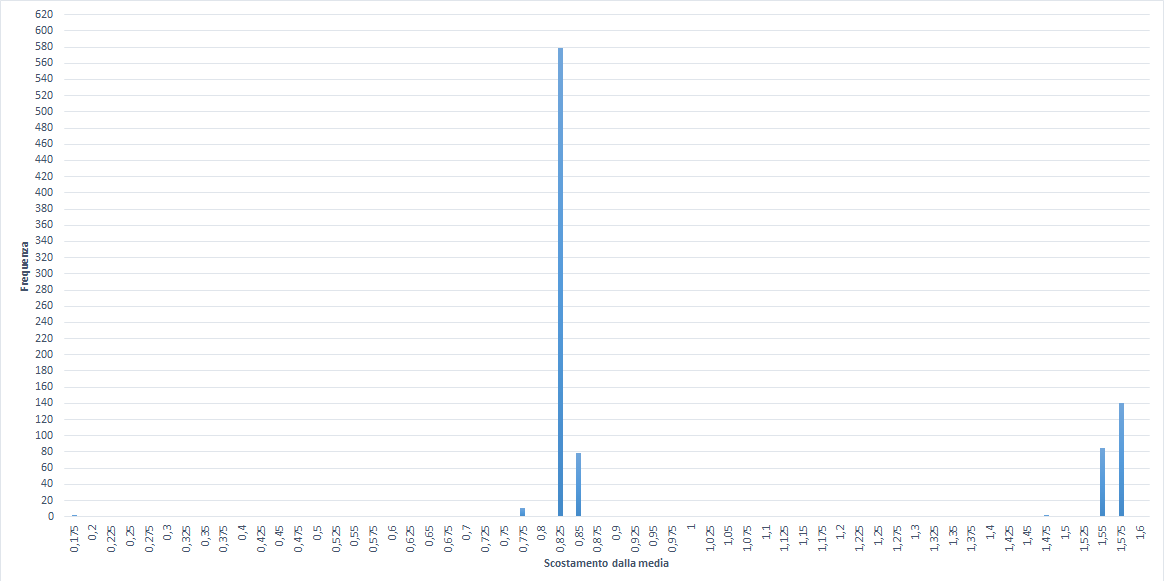
\includegraphics[scale=.35]{cap5/misfisso1b}}
\caption{Misure a bersaglio fisso con finestratura rettangolare}\label{misfisso1}
%% TODO Cap5: qui le misure sono 900 e non 1000!
\end{figure}

\begin{figure}
\centering
\subfigure[Misure di distanza e media]
{\label{misfisso2a}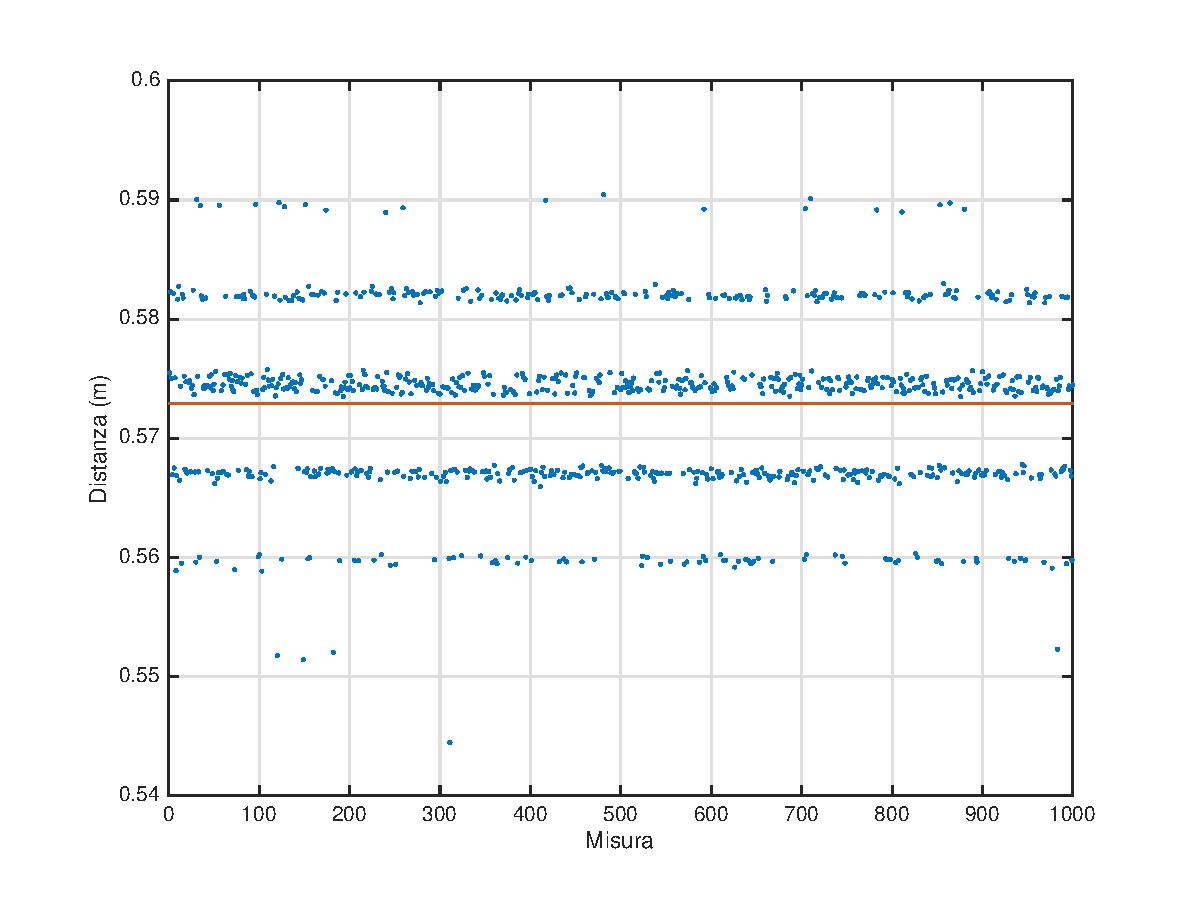
\includegraphics[scale=.5]{cap5/misfisso2a}}
\hspace{5mm}
\subfigure[Distribuzione dei valori misurati rispetto alla media]
{\label{misfisso2b}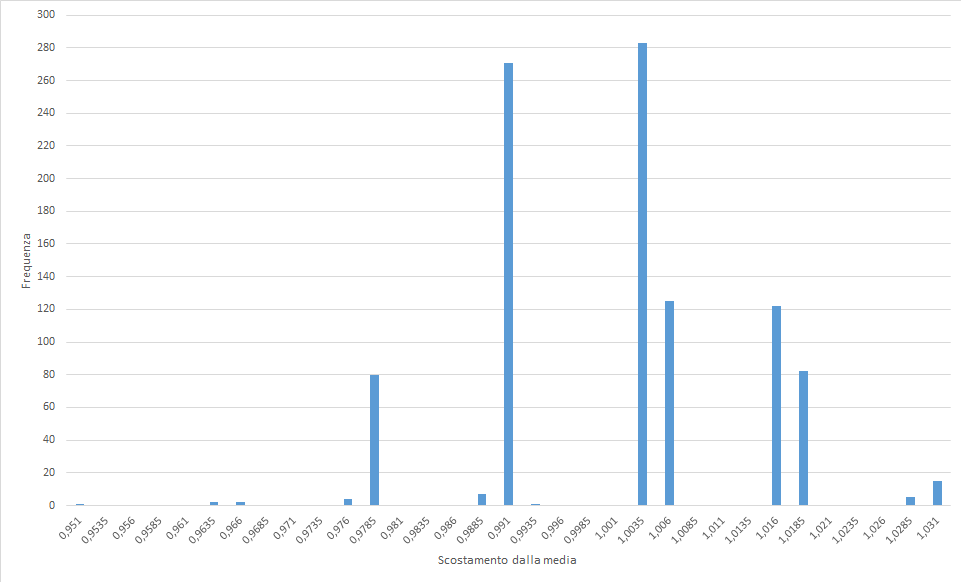
\includegraphics[scale=.5]{cap5/misfisso2b}}
\caption{Misure a bersaglio fisso con finestratura di Hanning}\label{misfisso2}
\end{figure}

\begin{figure}
\centering
\subfigure[con finestra rettangolare]
{\label{mismobile1}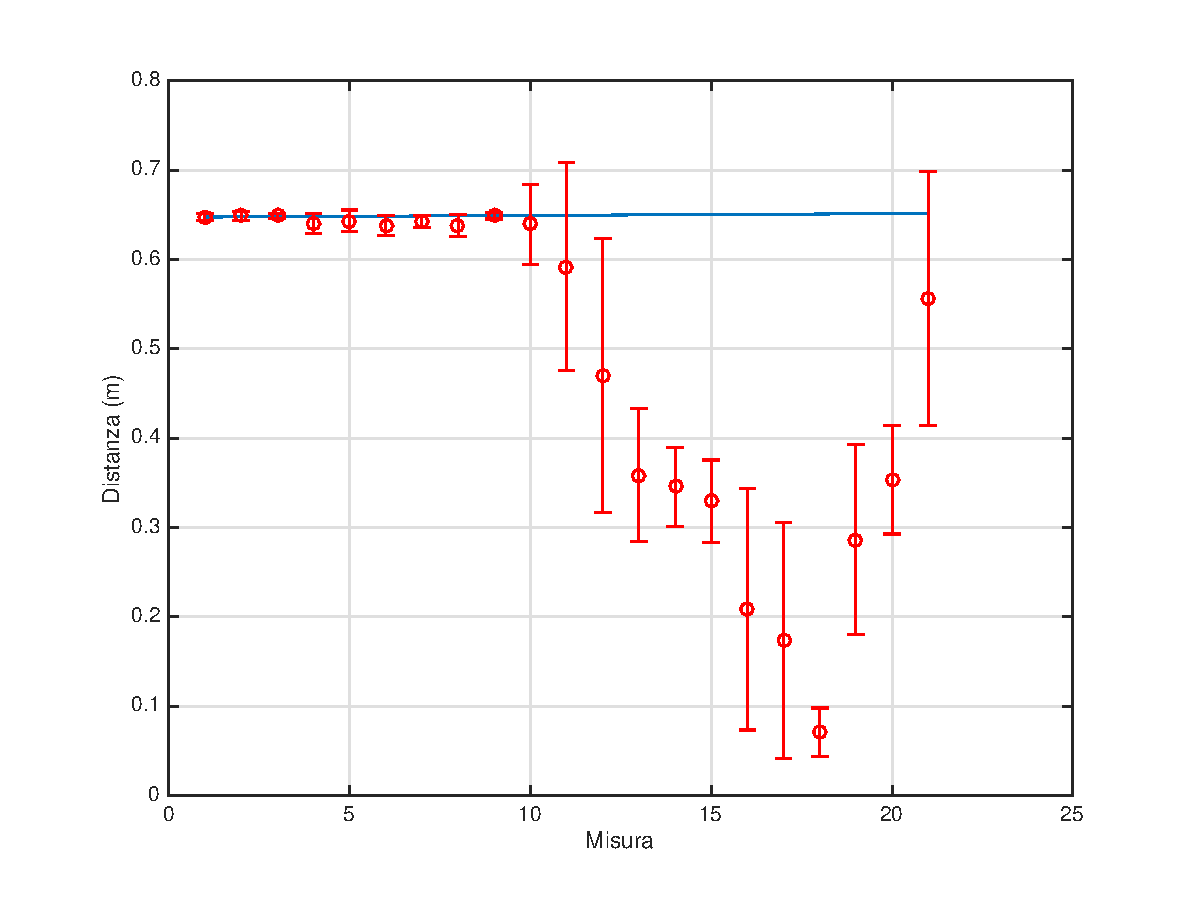
\includegraphics[scale=.5]{cap5/mismobile1}}
\hspace{5mm}
\subfigure[con finestra di Hanning]
{\label{mismobile2}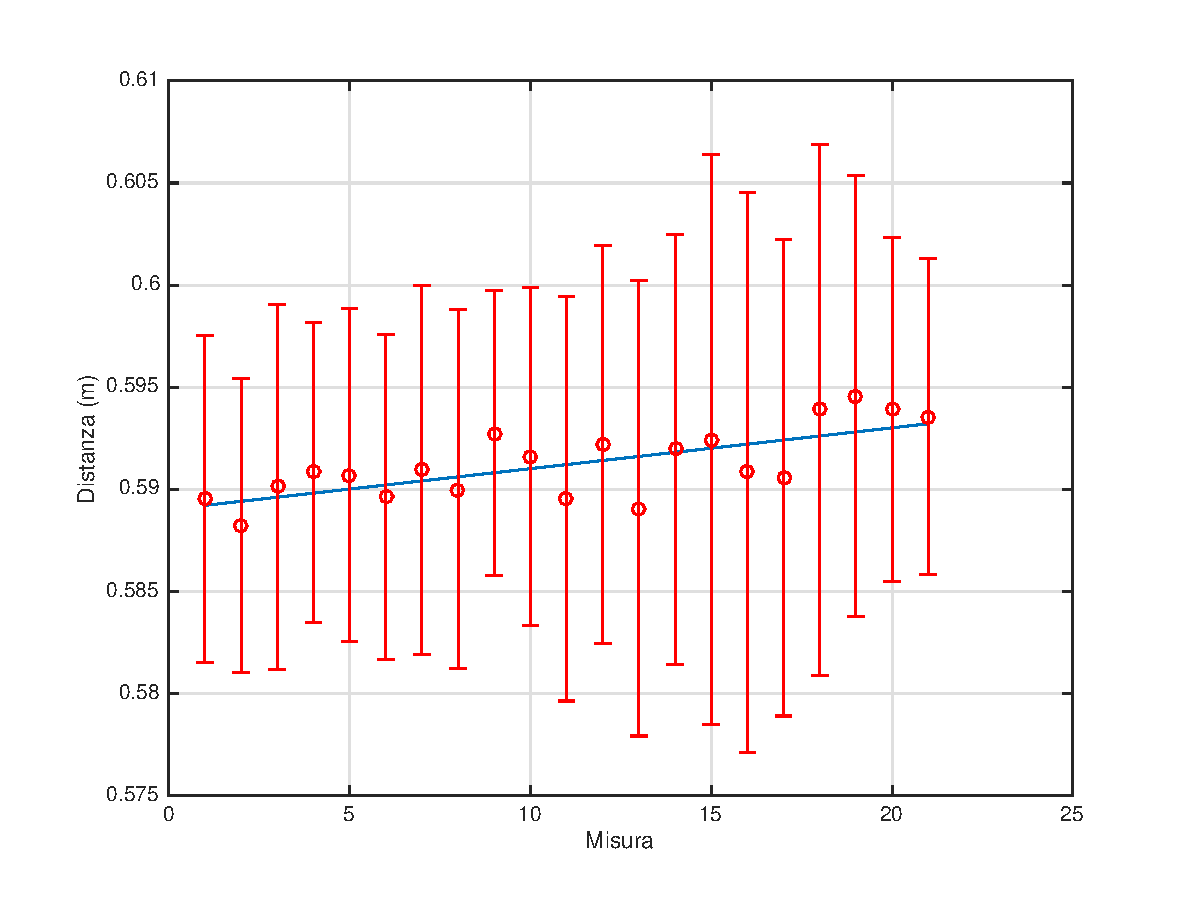
\includegraphics[scale=.5]{cap5/mismobile2}}
\caption{Misure di distanza a bersaglio mobile effettuate su $200 \mu m$ di spostamento}\label{mismobile12}
\end{figure}

I risultati delle prove a bersaglio fisso sono mostrati in Figura \ref{misfisso1} e \ref{misfisso2}. Sono inoltre riportati i grafici della distribuzione dei punti misurati rispetto alla media. In figura \ref{mismobile12}, invece, sono mostrate le misure a bersaglio mobile: i punti rossi rappresentano le medie valutate ogni $100$ misurazioni, e le barre di errore l'incertezza assoluta di misura. La curva blu, invece, rappresenta il valore atteso.

Dai risultati delle misure a bersaglio fisso si evince che con la finestratura di \textit{Hanning} vi è un chiaro miglioramento in termini di precisione. L'incertezza relativa di misura si riduce complessivamente di un fattore $10$ passando da $10^{-1}$, con finestra rettangolare, a $10^{-}2$ con finestra di \textit{Hanning}.

Si nota inoltre, dai risultati delle misure a bersaglio mobile, che l'utilizzo della finestra di \textit{Hanning} rende lo strumento lineare allo spostamento con un errore massimo picco-picco dell'ordine del millimetro (ca. $4mm$). \'E facile intuire graficamente che l'utilizzo della finestra rettangolare rende lo strumento fortemente non lineare allo spostamento.
\begin{figure}  
  \begin{center}
    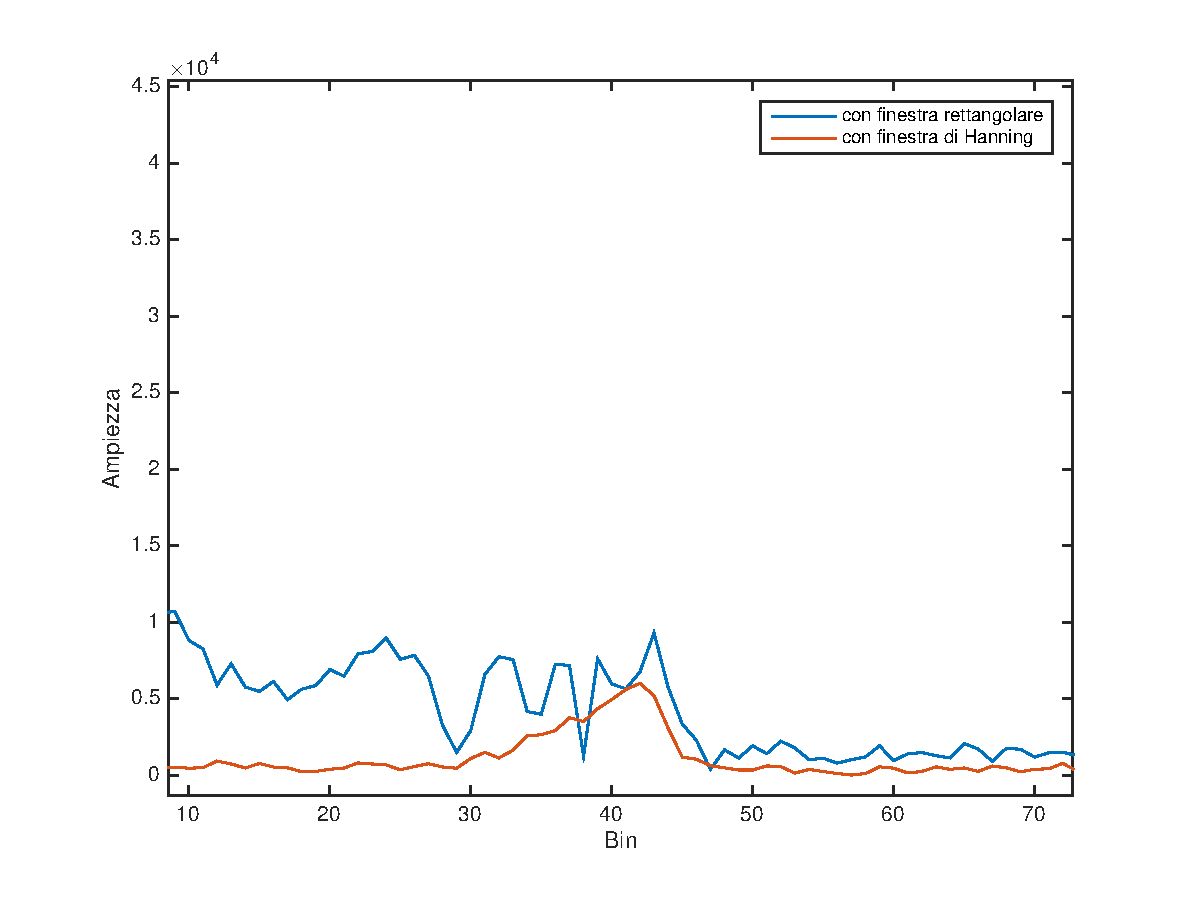
\includegraphics[scale=0.5]{cap5/spectleakinterf}
    \caption{Porzione di spettro calcolato sul fronte di discesa dalla FFT con finestra rettangolare e di Hanning}
    \label{spectleakinterf}
  \end{center}
\end{figure}

Il motivo che spiega questo miglioramento è la diminuzione dello \textit{spectral leakage}, che risulta meno marcato per la finestra di \textit{Hanning} piuttosto che per quella rettangolare. In figura \ref{spectleakinterf} sono confrontati gli spettri di frequenza di un segnale interferometrico calcolati sul fronte di discesa dalla FFT con finestra rettangolare e di \textit{Hanning}. Dalla figura si nota l'evidente effetto dello \textit{spectral leakage} che affligge la FFT con finestra rettangolare.

\section{Linearizzazione della misura}
Nonostante i notevoli miglioramenti in termini di precisione, il misuratore possiede ancora una scarsa accuratezza. Tale limitazione dipende dalla lunghezza del periodo di frangia del segnale interferometrico. In particolare, fissata la distanza $s$ dell'ostacolo e modulando triangolarmente il laser, quindi con pendenza $\frac{\Delta I}{\Delta t}$ costante, il periodo di frangia $t_{frangia}$ dovrebbe essere costante lungo tutto il segnale. 
\begin{figure}  
  \begin{center}
    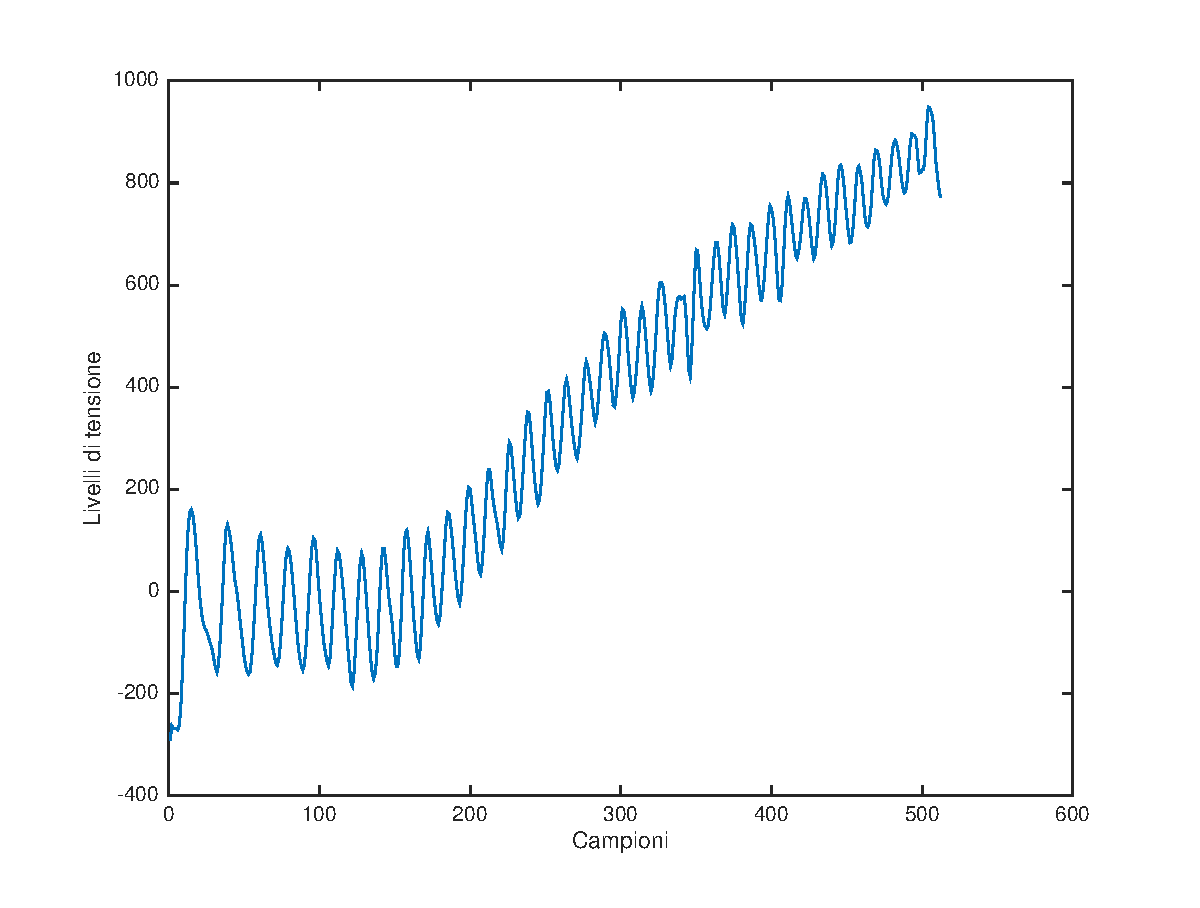
\includegraphics[scale=0.5]{cap5/semiperiodononcomp}
    \caption{Semiperiodo del segnale interferometrico prodotto dalla sorgente laser con modulazione a pendenza $\frac{\Delta I}{\Delta t}$ costante su di un bersaglio metallico a distanza fissa}
    \label{semiperiodononcomp}
  \end{center}
\end{figure}

Tuttavia, come osservato in Figura \ref{semiperiodononcomp}, il periodo della singola frangia $t_{frangia}$ non è costante lungo tutto il fronte di salita o di discesa. Di conseguenza, questo fenomeno è la causa del limite sull'accuratezza della misura.

Questo limite sull'accuratezza è dovuto alla non-linearità del laser. È possibile notare dall'equazione utilizzata per il calcolo della distanza assoluta: 
\begin{equation}
	s = \frac{\lambda^2}{2\left ( \frac{\Delta I}{\Delta T} \frac{\Delta \lambda}{\Delta I} \right ) t_{frangia}} 
\end{equation}
che è il parametro $\chi = \frac{\Delta \lambda}{\Delta I}$ a causare la non-linearità del periodo di frangia. Infatti dal momento in cui tutti i parametri sono fissati, l'unico che può causare la non-linearità è appunto $\chi$.

Un secondo motivo per cui il tempo di frangia $t_{frangia}$ non è costante è la costante termica del laser, che causa un ritardo nel raggiungimento di una condizione di equilibrio.

Queste caratteristiche sono peculiari della sorgente, e sono esclusivamente dipendenti dalla frequenza di modulazione della corrente.	

I due effetti combinati, quindi, causano una non linearità nella frequenza delle frange; in particolare le frange che si trovano all'inizio del segnale interferometrico sono a frequenza più bassa di quelle alla fine.	

\subsection{Metodo di compensazione della non-linearità}
Una tecnica per compensare le variazioni del parametro $\chi = \frac{\Delta \lambda}{\Delta I}$ consiste nell'utilizzare un segnale modulante con pendenza $\frac{\Delta I}{\Delta t}$ variabile durante il semiperiodo di modulazione. Per fare ciò è necessario ricavare l'andamento $\chi = \frac{\Delta \lambda}{\Delta I}$ conoscendo quello del $t_{frangia}$ o, in alternativa, $f_{frangia}$. Una volta ricavato l'andamento non-lineare nel tempo di $\chi = \frac{\Delta \lambda}{\Delta I}$ lo si compensa, modificando $\frac{\Delta I}{\Delta t}$, in modo che il prodotto $\frac{\Delta I}{\Delta t} \frac{\Delta \lambda}{\Delta I}$ sia costante e, di conseguenza, anche $t_{frangia}$ risulti costante.

Il metodo utilizzato per ricavare la forma d'onda del segnale di modulazione è stato implementato in LabVIEW Real-Time ed eseguito sul microprocessore della scheda di prototipazione. Per permettere ciò, è stato utilizzato un firmware FPGA, leggermente diverso de quello implementato nello strumento finale, che permettesse di inviare al microprocessore il segnale interferometrico completo e non solo i risultati dell'algoritmo di FFT.

Di seguito vengono descritti i passi principali del metodo di compensazione sviluppato:
\begin{figure}  
  \begin{center}
    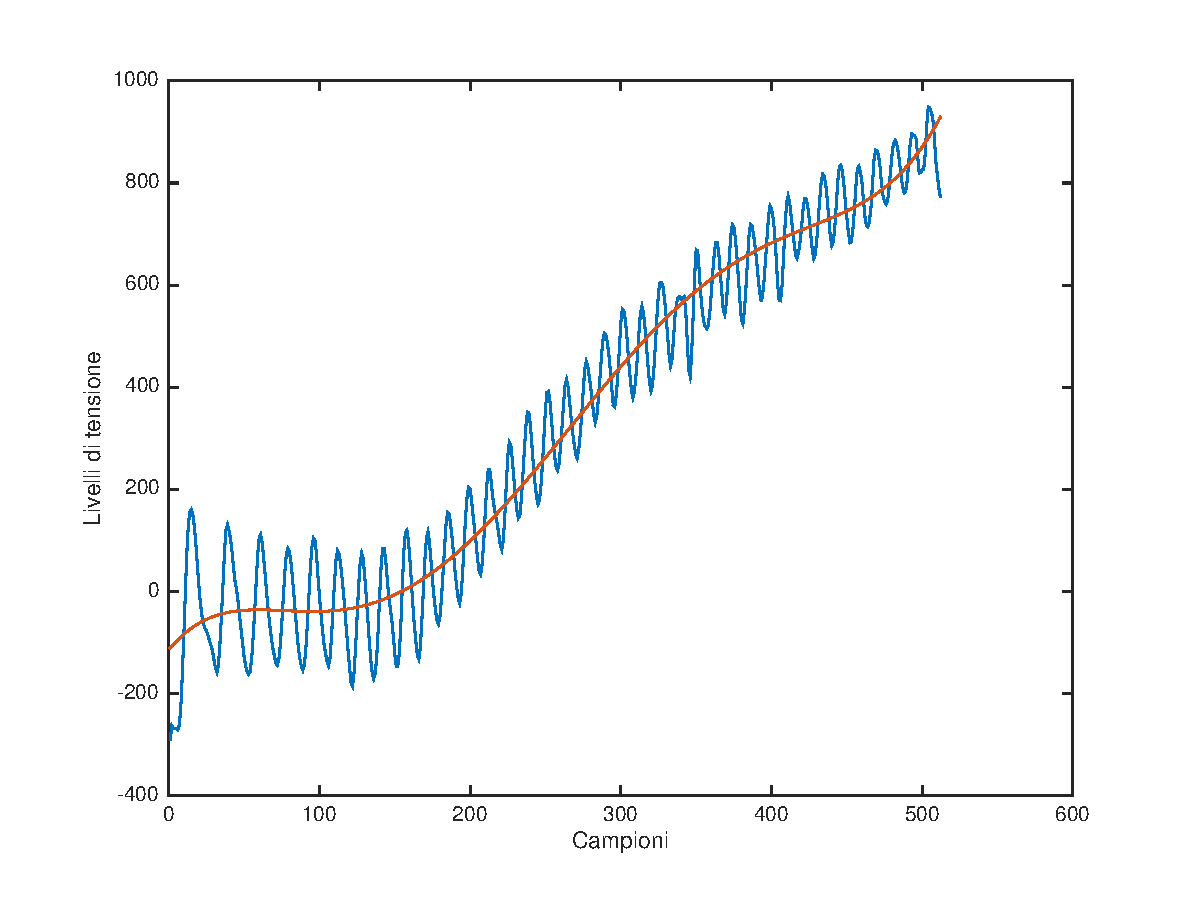
\includegraphics[scale=0.5]{cap5/regressioncurvefrangia}
    \caption{Curva di regressione polinomiale del segnale interferometrico}
    \label{regressioncurvefrangia}
  \end{center}
\end{figure}

\begin{figure}  
  \begin{center}
    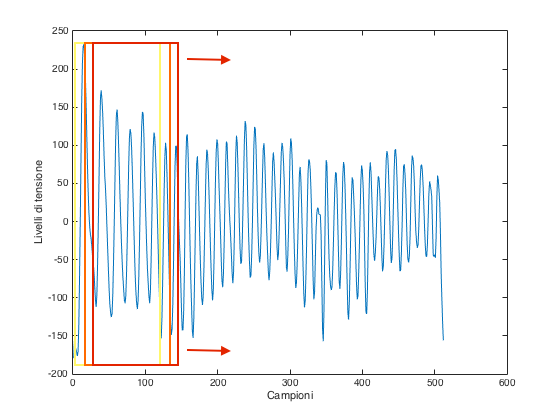
\includegraphics[scale=0.5]{cap5/slidingfft}
    \caption{Spostamento della finestra di 128 campioni lungo il semiperiodo di modulazione su cui viene calcolata la FFT}
    \label{slidingfft}
  \end{center}
\end{figure}

\begin{figure}  
  \begin{center}
    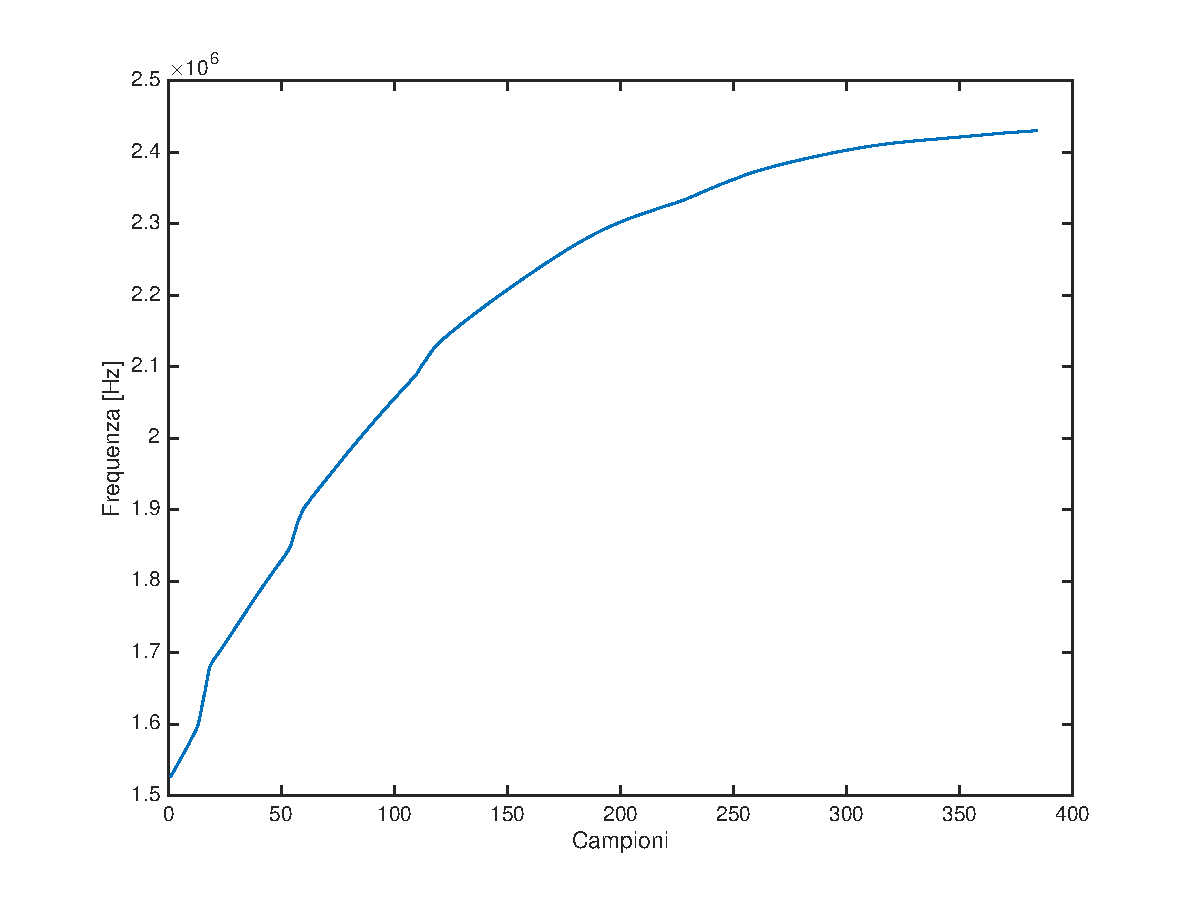
\includegraphics[scale=0.5]{cap5/curvamediatafreq}
    \caption{Curva mediata delle frequenze in un semiperiodo di modulazione con ostacolo a distanza fissa}
    \label{curvamediatafreq}
  \end{center}
\end{figure}

\begin{figure}
\centering
\subfigure[Semiperiodo di discesa]
{\label{}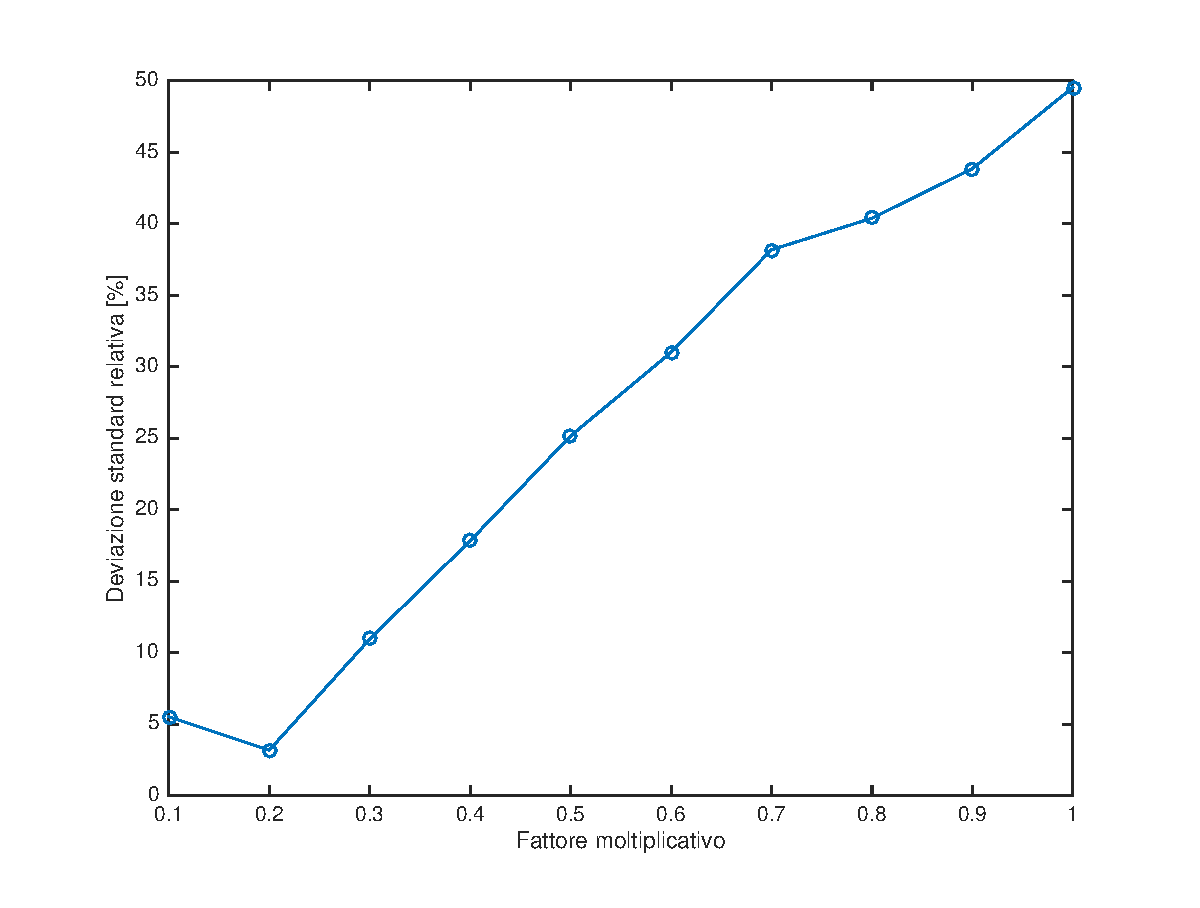
\includegraphics[scale=.3]{cap5/mulfactdiscesa}}
\hspace{5mm}
\subfigure[Semiperiodo di salita]
{\label{}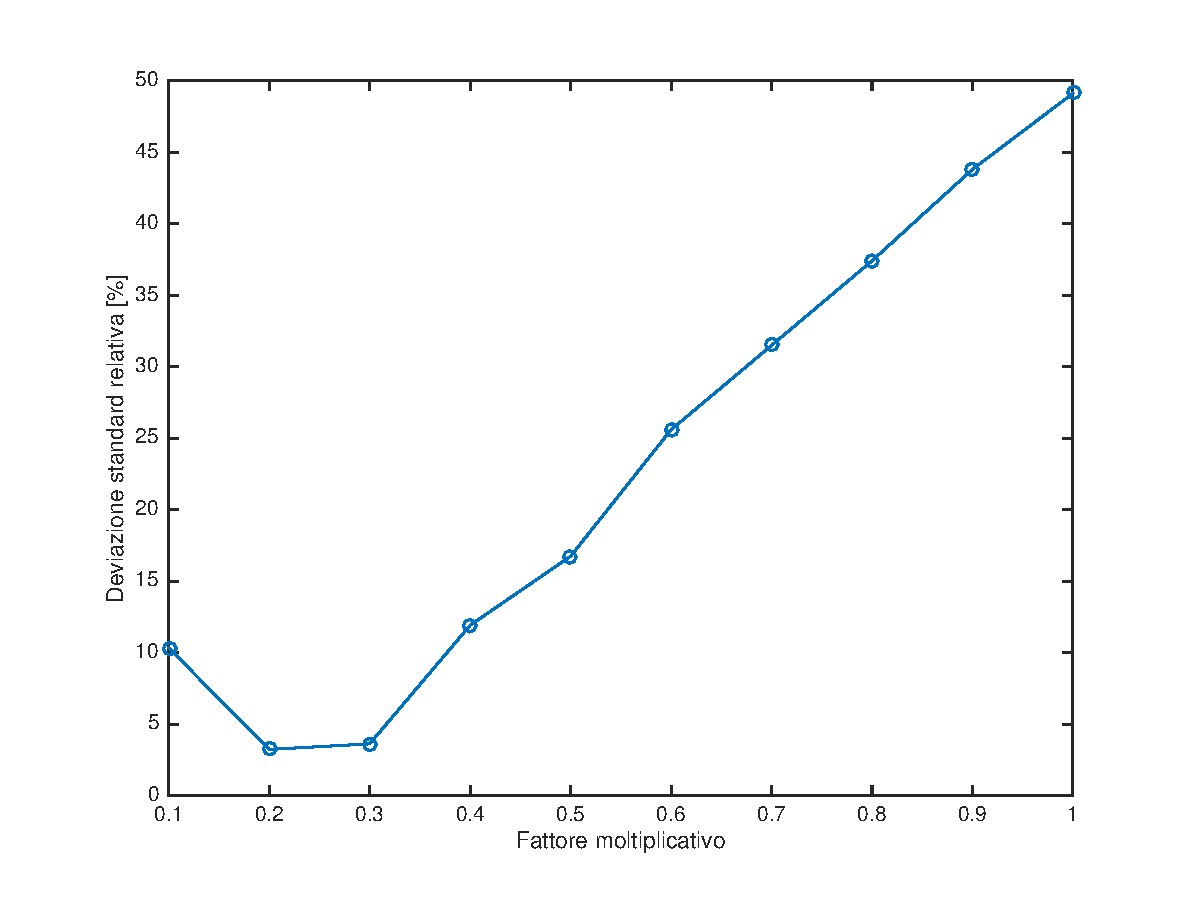
\includegraphics[scale=.3]{cap5/mulfactsalita}}
\caption{Curva delle deviazioni standard relative dei due fronti al variare del fattore moltiplicativo}\label{mulfact}
\end{figure}

\begin{enumerate}
	\item \underline{Modulazione triangolare}: La forma d'onda utilizzata per la modulazione è un'onda triangolare simmetrica con pendenza fissa. Il bersaglio è posto ad un distanza tale da produrre un elevato numero di frange (nel nostro caso si è posto il bersaglio a circa $50cm$ dal sensore).
	\item \underline{Calcolo della curva di regressione polinomiale}: Per avere una misura più precisa delle frequenza di frangia è stata calcolata la curva di regressione polinomiale di grado $5$ del segnale interferometrico (esempio in Figura \ref{regressioncurvefrangia}) ed è stata sottratta digitalmente da esso. In questo modo la lunghezza del tempo di frangia è valutata in modo più rigoroso.
	\item \underline{Calcolo della curva delle variazione delle frequenze di frangia}: L'algoritmo analizza separatamente i due fronti, ricevendo in ingresso i $512$ campioni del segnale interferometrico per ciascun fronte. Per ogni fronte si selezionano i primi $128$ campioni e si estrae il valore di frequenza corrispondente alle prime frange del segnale. Per l'estrazione della frequenza del segnale, LabVIEW offre un metodo già implementato chiamato \textit{Extract Single Tone Information}. Si tratta di una FFT con finestra di \textit{Hanning} interpolata a due punti, con una correzione per l'aliasing intorno alla continua a $\frac{f_{sample}}{2}$. A questo punto la finestra di selezione viene traslata di un campione verso destra e la frequenza delle frange viene ricalcolata (Figura \ref{slidingfft}). Questa operazione viene effettuata fino a che la selezione comprende l'ultimo campione del segnale interferometrico.
	
	In questo modo si ottengono $384$ valori di frequenze per ciascun fronte, in funzione della posizione delle frange all'interno del fronte stesso (Figura \ref{curvamediatafreq}). Questo procedimento è stato effettuato per $100$ segnali acquisiti ed i risultati sono stati poi mediati. \'E stato deciso di associare ai primi $113$ ($=625-512$) campioni scartati valori di frequenza fittizi, approssimando tali valori con una retta di pendenza pari alla pendenza della prima frequenza estratta, mentre agli ultimi $128$ ($=512-384$) campioni è stata associata una retta con pendenza pari alla pendenza dell'ultima frequenza estratta.
	\item \underline{Calcolo iterativo del fattore moltiplicativo} \underline{da applicare alla curva delle} \underline{frequenze}: La curva mediata delle frequenze, ricavata al passo precedente, viene moltiplicata alla triangolare con pendenza costante ricavando così il segnale di modulazione con pendenza $\frac{\Delta I}{\Delta t}$ non costante.
	
	Da verifiche sperimentali è nata la necessità di moltiplicare i semiperiodi della curva di modulazione per un fattore di scala, che è stato scelto in modo che la deviazione standard relativa delle frequenze rilevate dall'FFT a scorrimento sia la minore possibile.
	
	Questo fattore viene ricavato iterativamente. Partendo da un valore $1$ e diminuendo il fattore di scala di passi di $0.1$ fino ad arrivare a $0$, si calcola la deviazione standard relativa delle frequenze estratte dall'FFT a scorrimento e si sceglie il fattore di scala che la minimizza.
	
	Questo procedimento è stato reiterato una seconda volta aumentando il numero di cifre significative del fattore di scala stesso (partendo da $0.35$ ed arrivando a $0.15$ con passi di $0.01$), in modo da aumentare la precisione della linearizzazione.
	
	Le prime curve ricavate vengono presentate in Figura \ref{mulfact}. Si può notare che sia per il fronte di salita che per il fronte di discesa il minimo si trova nell'intorno di $0.2$. I valori esatti ricavati nella seconda iterazione sono $0.18$ per il fronte di discesa e $0.22$ per il fronte di salita.
	\item \underline{Generazione della curva di modulazione compensata}: La curva delle frequenze, scalata dei valori moltiplicativi calcolati al passo precedente, viene moltiplicata alla triangolare con pendenza costante ricavando così il segnale di modulazione con pendenza $\frac{\Delta I}{\Delta t}$ non costante.	
\end{enumerate}
\begin{figure}  
  \begin{center}
    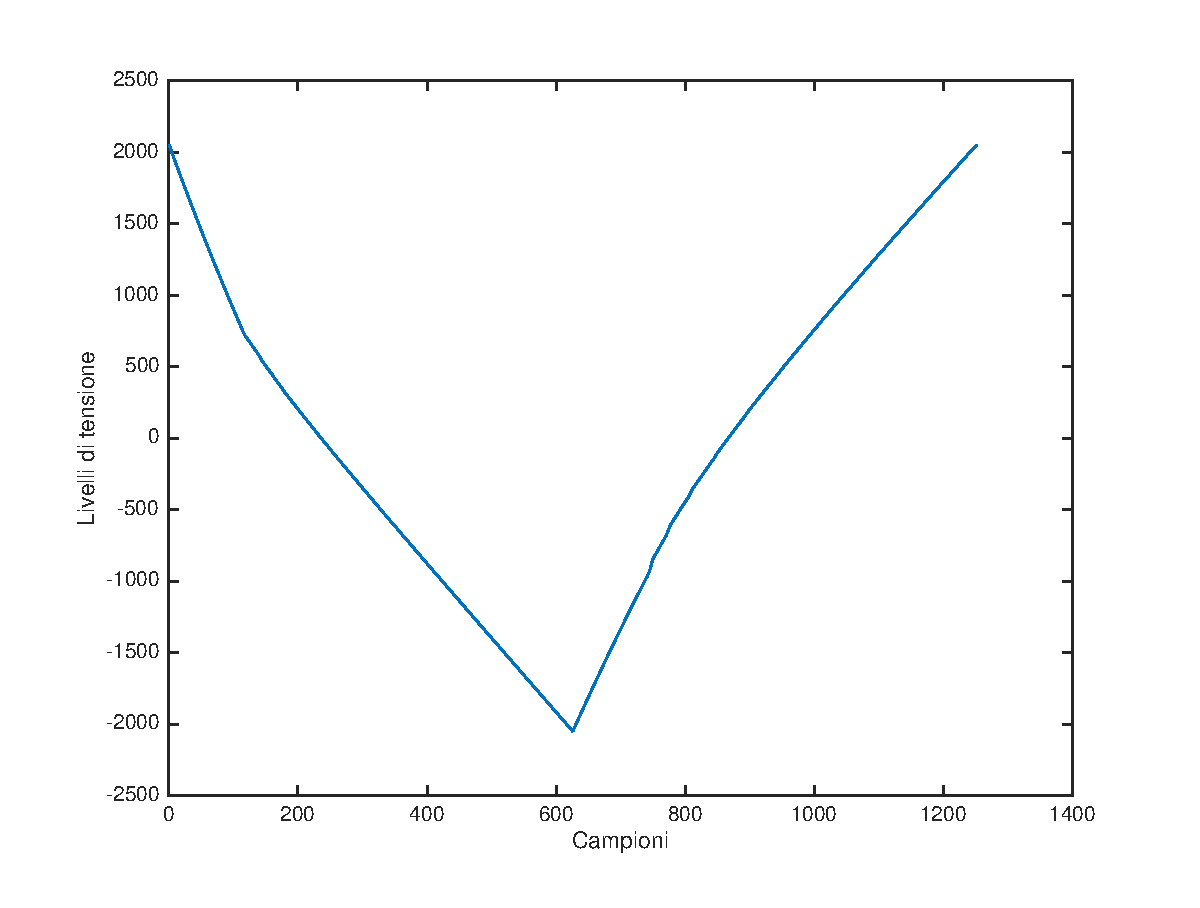
\includegraphics[scale=0.5]{cap5/ondafinale}
    \caption{Forma d'onda finale usata per la modulazione}
    \label{ondafinale}
  \end{center}
\end{figure}

La forma d'onda finale, mostrata in Figura \ref{ondafinale}, ha consentito di ridurre la dispersione del $t_{frangia}$, migliorando l'accuratezza della misura di distanza. La pendenza iniziale sia nel fronte di salita che in quello di discesa è accentuata rispetto alla triangolare originaria, come era prevedibile dallo studio in frequenza. Infatti la frequenza di frangia presentava un andamento monotono crescente al variare della corrente di modulazione, effetto compensato dall'aumento della pendenza nella triangolare compensata.

\subsection{Misure in seguito alla compensazione}
Al fine di valutare la bontà dell'algoritmo precedentemente descritto, è stata comparata quantitativamente l'incertezza relativa della variazione di frequenza del segnale interferometrico prima e dopo la compensazione del segnale di modulazione.

\begin{figure}
\centering
\subfigure[Semiperiodo di discesa]
{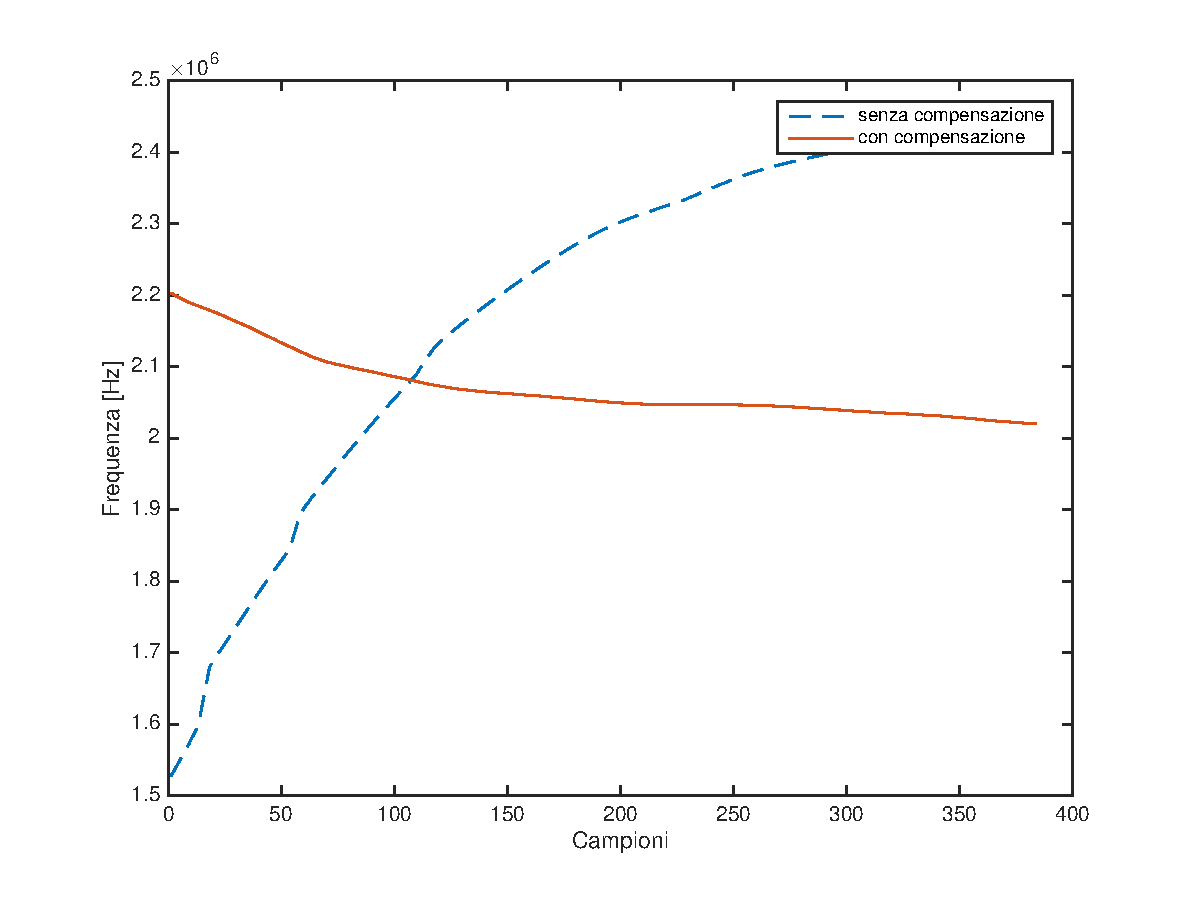
\includegraphics[scale=.3]{cap5/primadopocompdisc}}
\hspace{5mm}
\subfigure[Semiperiodo di salita]
{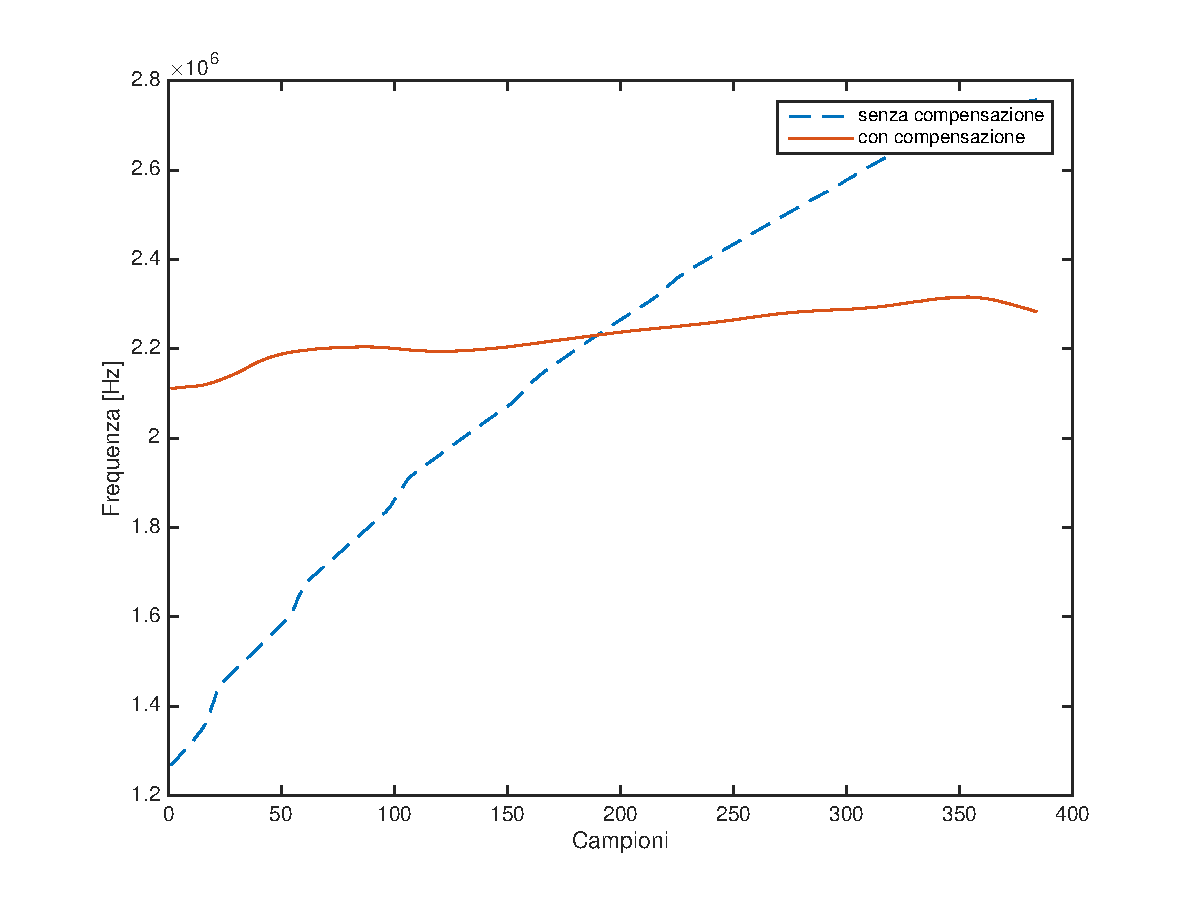
\includegraphics[scale=.3]{cap5/primadopocompsal}}
\caption{Curve mediate delle frequenze estratte per entrambi i fronti di modulazione, prima e dopo la compensazione}\label{primadopocomp}
\end{figure}

I miglioramenti ottenuti per merito della compensazione della non-linearità sono mostrati in figura \ref{primadopocomp}. Dalle prove sperimentali è emerso che l'incertezza relativa della variazione di frequenza, valutata su $100$ semiperiodi di modulazione, è scesa intorno al $2\%$, per entrambi i fronti di modulazione, contro i $20\%$ ottenuti senza compensazione. La prova è stata ripetuta più volte per verificare che il guadagno in termini di linearità del periodo di frangia sia effettivamente $10$.
\begin{figure}
\centering
\subfigure[Misure di distanza e media]
{\label{misfisso3a}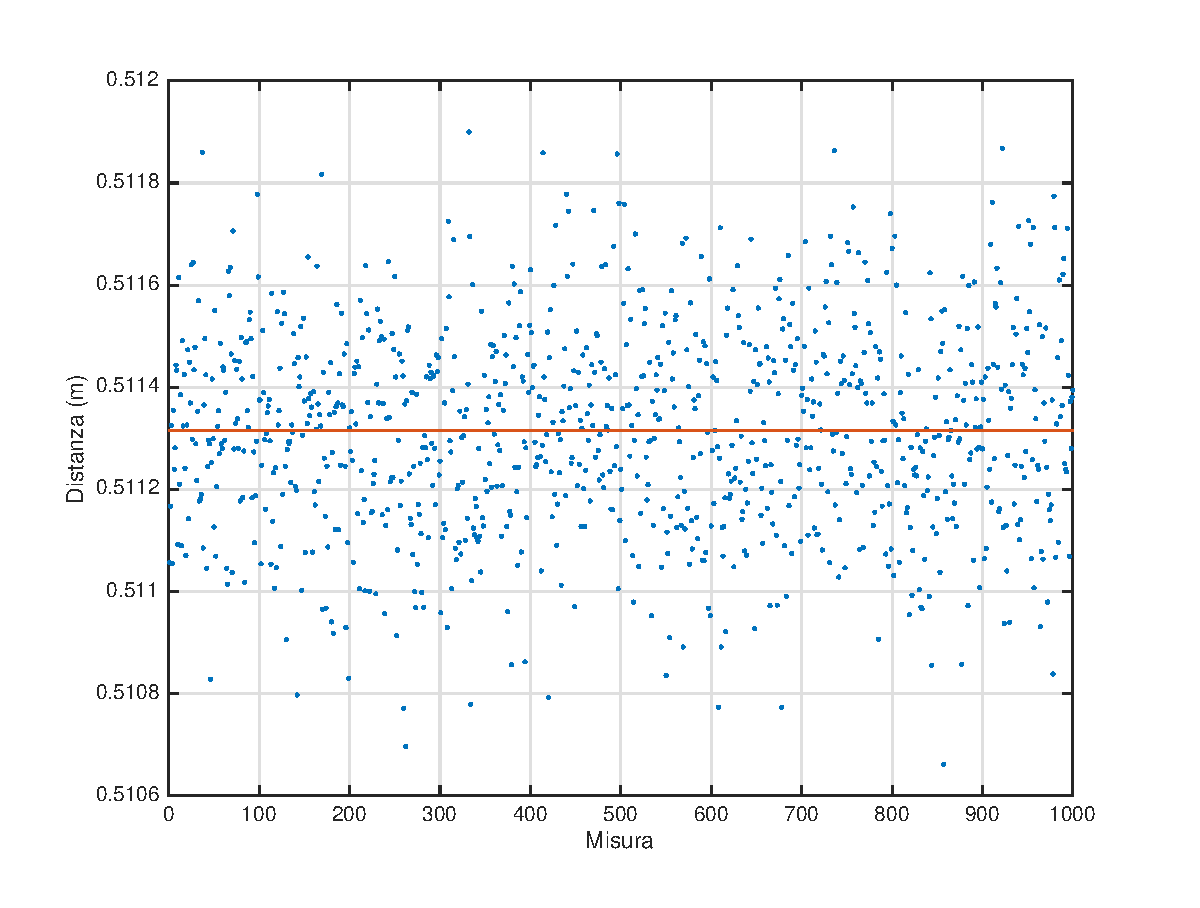
\includegraphics[scale=.5]{cap5/misfisso3a}}
\hspace{5mm}
\subfigure[Distribuzione dei valori misurati rispetto alla media]
{\label{misfisso3b}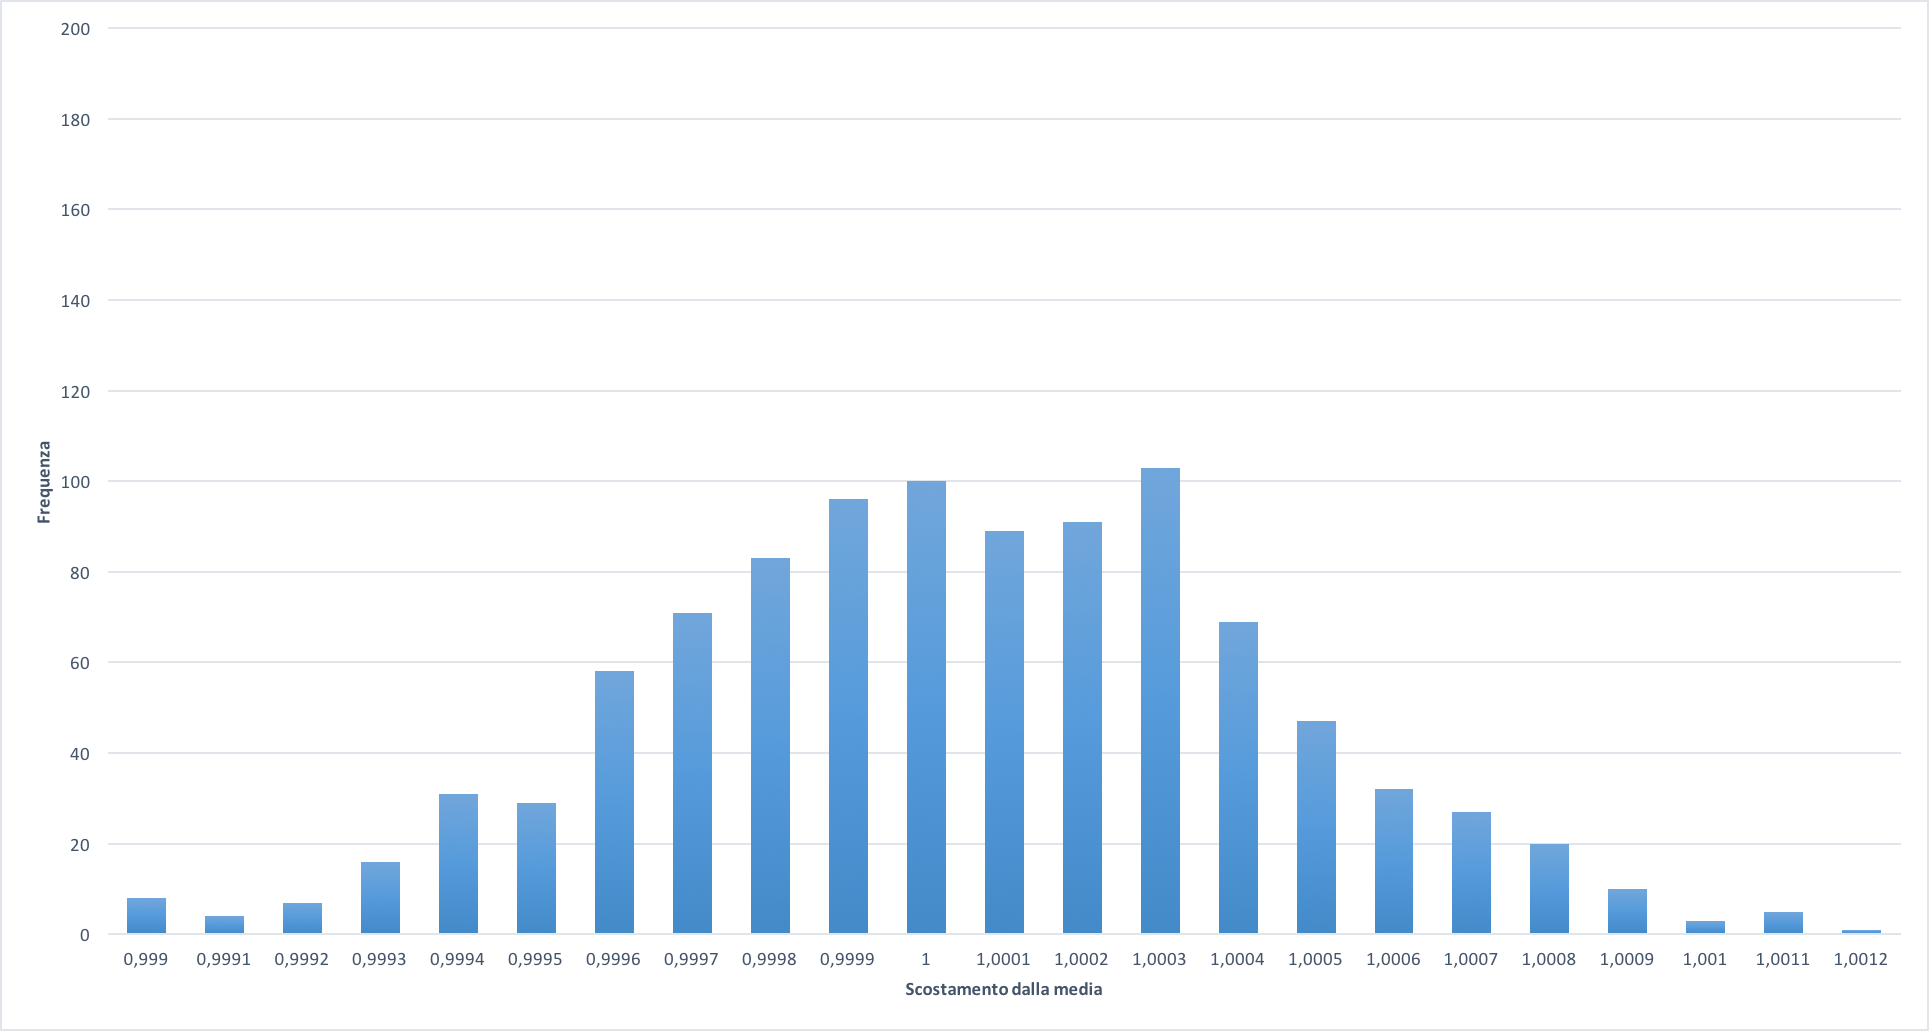
\includegraphics[scale=.4]{cap5/misfisso3b}}
\caption{Misure a bersaglio fisso con segnale di modulazione compensato}\label{misfisso3}
\end{figure}

\begin{figure}  
  \begin{center}
    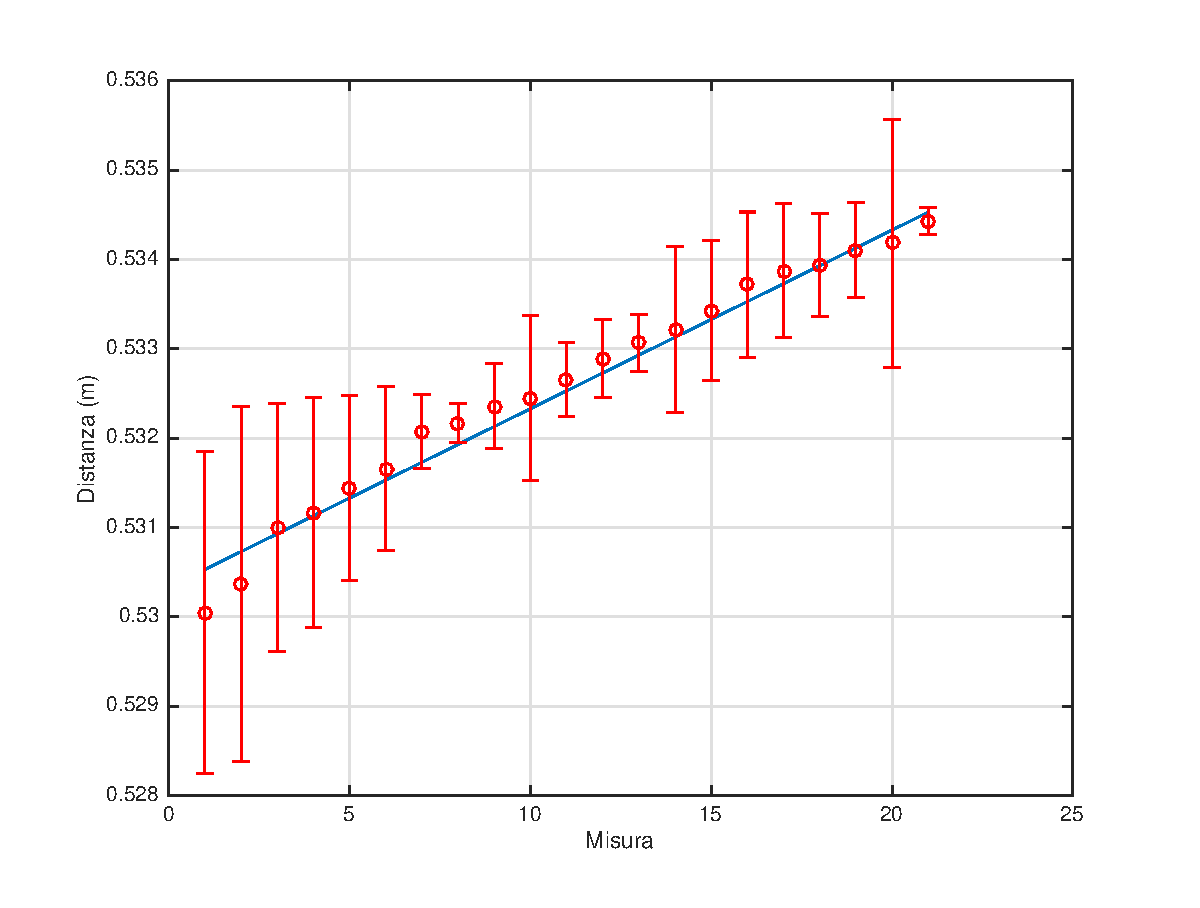
\includegraphics[scale=0.5]{cap5/mismobile3}
    \caption{Misure di distanza a bersaglio mobile effettuate su $200\mu m$ di spostamento con segnale di modulazione compensato}
    \label{mismobile3}
  \end{center}
\end{figure}

Questo miglioramento ha influito sulla precisione e sull'accuratezza della misura. A conferma del risultato sono riportati gli esiti delle prove a bersaglio fisso e a bersaglio mobile rispettivamente in figura \ref{misfisso3} e \ref{mismobile3}.

Si può apprezzare, dai risultati delle misure a bersaglio fisso, che utilizzando un segnale di modulazione compensato la precisione di misura migliora sensibilmente. In particolare, l'incertezza relativa diminuisce di due ordini di grandezza, passando da $10^{-2}$ a $4 \cdot 10^{-4}$.

Inoltre, si può notare come le misure effettuate con la modulazione compensata risultino complessivamente più lineari rispetto a quella effettuata senza compensazione.

La valutazione dell'errore massimo picco-picco rispetto al valore atteso conferma quanto intuito graficamente: l'errore nel caso di segnale di modulazione con pendenza compensata migliora discretamente passando da $4mm$ a $826 \mu m$, con un RMS pari a $568 \mu m$.

Nonostante l'ottimo miglioramento raggiunto, l'accuratezza non è ancora soddisfacente, a tal proposito si è ritenuto opportuno migliorare ulteriormente la misura con ottimizzazioni che verranno descritte nel paragrafo successivo.

\section{Ottimizzazione della misura}

\subsection{Variazione dell'ampiezza del segnale di modulazione}

\subsection{Sottrazione del residuo}

\section{Prove dello strumento finale}

\subsection{Bersaglio fisso}

\subsection{Bersaglio mobile}

\subsection{Range di misura}

\subsection{Prestazioni}

\section{Cenni su un'ulteriore ottimizzazione nell'algoritmo di compensazione}

\section{Drift termico}

\section{Precisazione sui risultati ottenuti}